\chapter{Implementación de la herramienta}
\label{cap:implementacion}

En esta sección se detallará la implementación de la herramienta, especificando cómo se ha implementado cada modulo y cada uno de los tests.  
Para la implementación de la herramienta se ha decidido utilizar \emph{C++} como lenguaje de programación. Para implementar el módulo de OCR, se ha decidido usar la librería Tesseract ya que proporciona api en \emph{C++}. Para facilitar el uso de la herramienta se ha decidido desplegar la aplicación en un contenedor. Como la aplicación se ejecuta dentro del entorno del contenedor, podemos usar la aplicación en cualquier sistema operativo. Para ello se ha decidido utilizar la herramienta de Docker\footnote{Docker \url{https://www.docker.com/}}.

Todo el material de la herramienta de testing de localización se encuentra en el repositorio de github\footnote{Repositorio de github de la herramienta:  \url{https://github.com/Dewo2000/TFG-2024-2025}}.

La herramienta de testing de localización tiene una arquitectura de clases como se muestra en la figura \ref{fig:UML}.
\begin{figure}[H]
	\centering
	\includegraphics[width = 1\textwidth]{Imagenes/TFGUml.pdf}
	\caption{Diagrama de clases de la herramienta.}
	\label{fig:UML}
\end{figure}
\section{Módulo de entrada}
Este es el módulo donde estará el programa principal donde se encarga de recibir los argumentos del usuario, parsear los argumentos, parsear los datos de configuración y llamar a los módulos de OCR y tests.
En el programa principal recibirá como parámetro:
\begin{itemize}
	\item --train. Para entrenar un modelo y se necesitará otros parametros para el entreno:
	\begin{itemize}
		\item -f font. Para especificar la fuente.
		\item -l lan. Para especificar el lenguaje.
		\item -i iter. El número de iteraciones.
		\item --clear . Si se elimina el entreno anterior del mismo modelo.
	\end{itemize}
	\item --test. Para hacer el test dada un archivo de configuración -c config.
\end{itemize}
Los datos proporcionados por el usuario son gestionados por la clase \texttt{LocalizationTests}, la cual se encarga de parsear los argumentos de entrada. En caso de que se indique un proceso de entrenamiento, esta clase invoca al módulo OCR en modo entrenamiento. Si, por el contrario, se trata de una ejecución de testing, se leerán del archivo de configuración los parámetros necesarios para llevar a cabo las pruebas.

\texttt{LocalizationTests} actúa como coordinadora entre los módulos principales del sistema: realiza las llamadas al OCR para el reconocimiento de texto y, una vez finalizado este proceso, organiza la ejecución de los tests de localización.

Los resultados de cada test son almacenados en un archivo en formato JSON, el cual se guarda en la ruta de salida especificada. Este archivo JSON puede ser interpretado posteriormente para generar un informe en formato HTML, cuyo proceso de conversión se detalla en la sección \ref{sec:Generación informe}.

A continuación se detalla la implementación de cada módulo.
\section{Implementación del modulo OCR}
\label{sec:Implementación del OCR}
En el modulo del OCR, tenemos principalmente dos partes, el entrenamiento del modelo y el reconocimiento de texto. Para la librería de OCR, en este caso se ha elegido Tesseract que cumple nuestras necesidades en tiempo y en precisión. La evaluación de las librerias de OCR se describe en la sección \ref{sec:Evaluación_OCR}.
\subsection{Entrenamiento de modelo}
Para el entrenamiento del modelo se ha usado la plantilla proporcionado por \cite{Joseda} donde se ha hecho el entreno usando la api de Tesseract en python. Para nuestro caso, hasta el día de la implementación, Tesseract no ha sacado ningún API para el entreno de modelo en \emph{C++}, por lo que en nuestra herramienta haremos llamadas al sistema con comandos proporcionado en la plantilla de \cite{Joseda} para el entreno de modelo.
\subsection{Reconocimiento de texto y mejoras}
Este módulo se ha diseñado pensando en su extensibilidad de modo que es posible usar otras librerías de OCR diferentes a la que se está usando la herramienta.
En este modulo es posible cambiar de libreria de OCR (p.ej EasyOCR) heredando de la clase virtual pura \texttt{OCR} y completando las funciones necesarias con métodos de esa librería sin afectar al funcionamiento completo de la herramienta. 

El proceso de reconocimiento y mejoras es el siguiente:
\begin{enumerate}
	\item  Recibidos parámetros del programa principal, este crea las carpetas correspondientes a la salida usando llamadas al sistema.
	\item Recorrerá la carpeta de imágenes preprocesando cada imagen con OpenCV.
	\item La imagen resultante del preprocesado será pasado a la librería de Tesseract para su reconocimiento de texto.
	\item Seguido de una limpieza de la salida de OCR usando la distancia Levenshtein en el caso de que el usuario haya proporcionado la salida esperada.
	\item  Al finalizar el proceso, escribirá la salida en el directorio de la salida con el formato \emph{nombre\_imagen.txt}.
\end{enumerate}
 
Para la recogida de parámetros, es necesario un archivo de configuración con el siguiente formato:
\begin{itemize}
	\item imagePath. Directorio donde se encuentra las imágenes.
	\item gtPath. Directorio donde se encuentra la cadena esperada de cada imagen.
   	\item model. Nombre del modelo que se va a usar.
	\item modelPath. Directorio donde se encuentra el modelo que se va a usar.
	\item outputPath. Directorio de salida de la información.
	\item OCR. El ocr que se va a usar. Por defecto Tesseract.
	\item placeholders. El formato de la cadena de placeholder que se usa. Debe tener un campo \texttt{begin} con la cadena de apertura del placeholder y un campo \texttt{end} con la cadena de cierre.
\end{itemize}

El preprocesado se ejecuta en el método protegido \texttt{preprocessing} de la clase \texttt{OCR}, la cual se usan métodos proporcionado por OpenCV de las cuales son:
\begin{itemize}
	\item \texttt{cvtColor} Cambia la imagen a escala de grises.
	\item \texttt{Resize}. Cambia las dimensiones la imagen, lo cual ajusta el tamaño de la imagen para un mejor reconocimiento.
	\item \texttt{Threshold} Aplica simple thresholding la cual asigna un valor binario a cada píxel dependiendo el umbral. Resalta mejor los caracteres del fondo.
	\item \texttt{fastNlMeansDenoising} Aplica reducción de ruido para mejorar la calidad visual y el reconocimiento.
	\item \texttt{medianBlur} y \texttt{GaussianBlur} Otra técnica para aplicar reducción de ruido suavizando la imagen.
	\item \texttt{dilate} y \texttt{erode} Técnica de dilatar y erosionar que ayuda a reducir ruidos y el cierre de contornos, mejora la detección de los caracteres.
	\item \texttt{createCLAHE} Ecualización adaptativa del histograma que mejora el contraste de la imagen.
\end{itemize}
La combinación anterior se ha obtenido haciendo estudio y experimento sobre las técnicas de preprocesamiento en la sección \ref{sec:Mejoras en el reconocimiento}.

El siguiente paso es el reconocimiento de texto utilizando la librería de Tesseract. El método \texttt{getDirImgText} para reconocer texto de una carpeta de imágenes se sitúa en la clase \texttt{OCR}, la cual es un método virtual puro que en la clase de \texttt{Tesseract} debe implementar. En el método se hace lo siguiente: 
\begin{enumerate}
	\item Genera las carpetas de salida relacionado al reconocimiento utilizando llamadas al sistema y dando permisos de escritura a la carpeta.
	\item Abre el directorio de carpetas con \texttt{opendir} y obteniendo la información en \texttt{dirent}, para obtener los nombres de los archivos y filtrar aquellas que son imágenes en formato png.
	\item Ejecutará el preprocesamiento de cada imagen con las técnicas anteriores.
	\item La imagen resultante será pasado al OCR con \texttt{SetImage} de Tesseract.
	\item Se obtendrá el texto reconocido con \texttt{GetUTF8Text} de Tesseract.
	\item Se hace la limpieza de caracteres utilizando distancia Levenshtein y se escribe en la salida el resultado.
\end{enumerate}
La limpieza se hace porque el OCR puede devolver caractéres basura(p.ej reconoce una caja del fondo como un carácter), y esta basura afecta a la detección de errores. Como por ejemplo, la figura \ref{fig:Ej.Basura} puede devolver
\begin{verbatim}
	"
	|
	\ J
	—
	Agumon /
	Still, a “smahrt fown” is cool! It really can
	do anything! <
\end{verbatim}
donde las primeras líneas son caracteres basura que ha reconocido el OCR.
\begin{figure}[H]
	\centering
	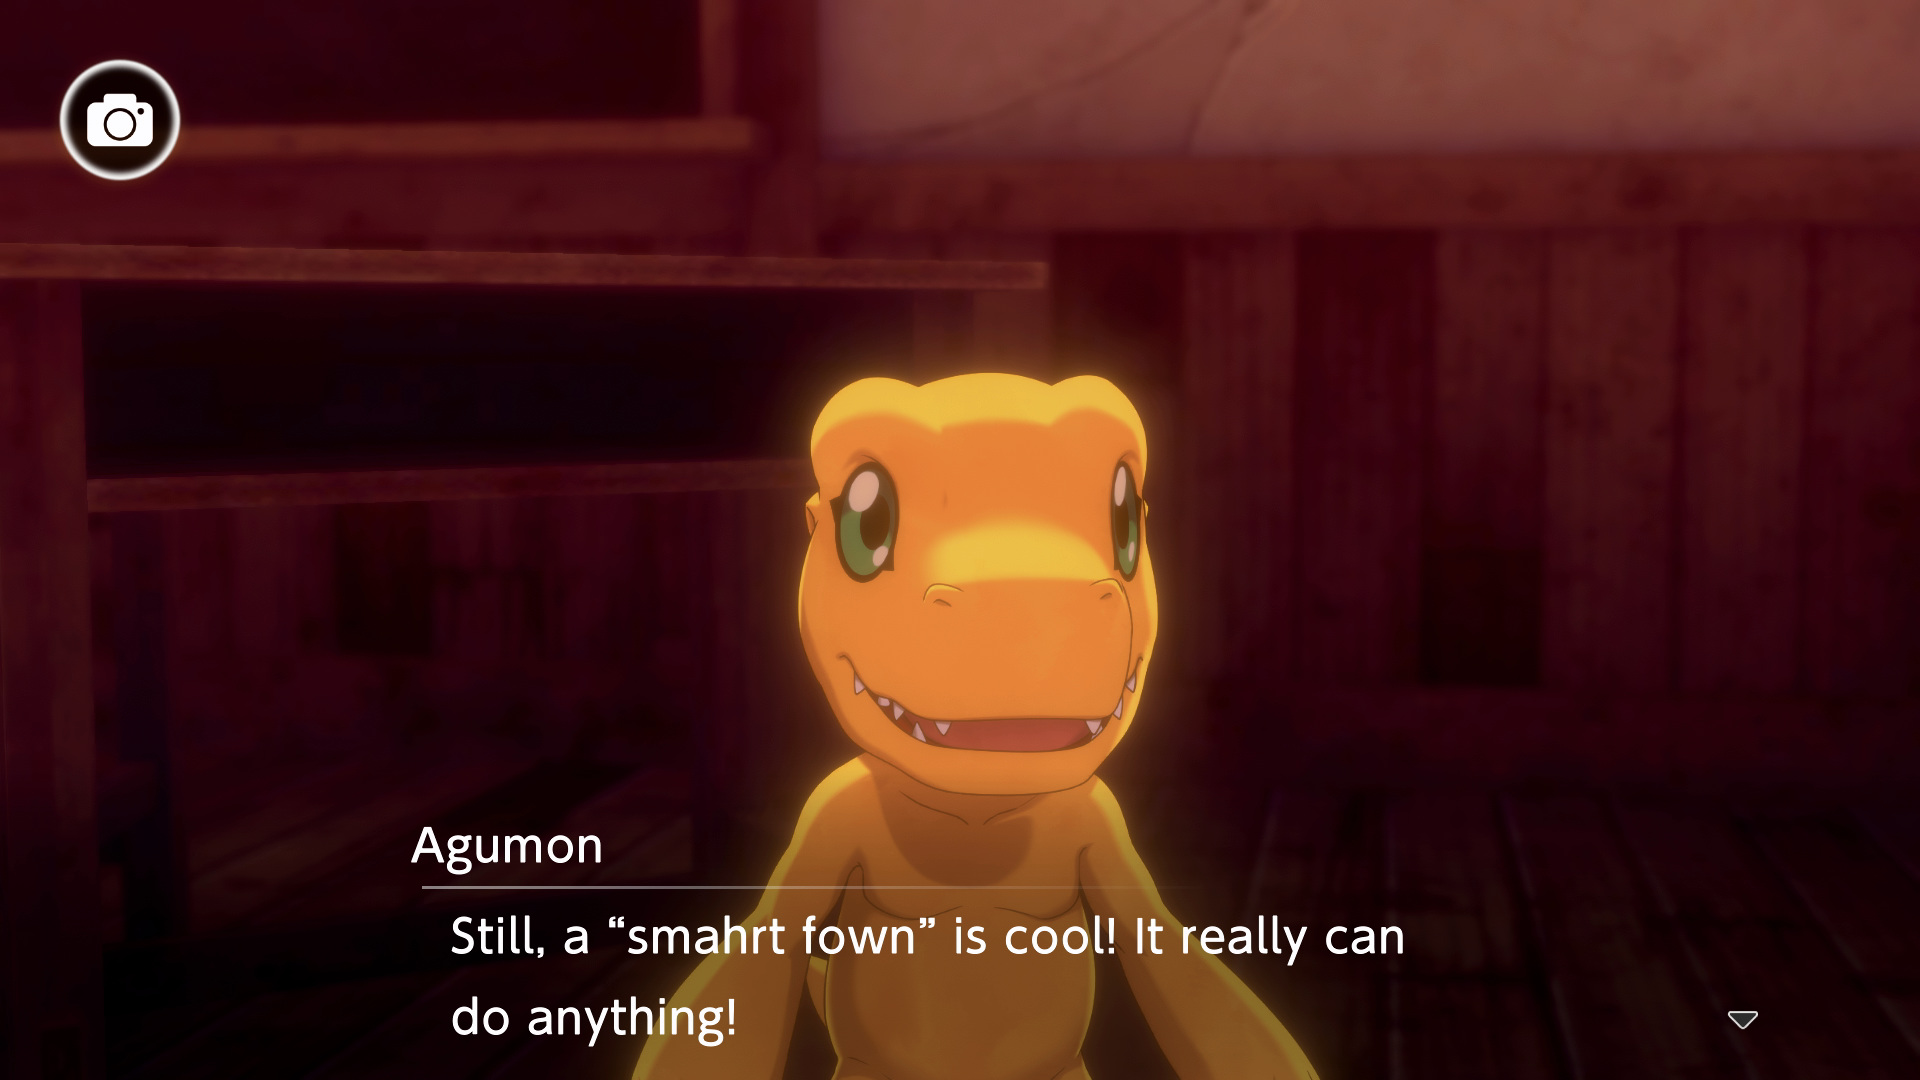
\includegraphics[width = 1\textwidth]{Imagenes/OCR/Simple.png}
	\caption{Diagrama de clases de la herramienta.}
	\label{fig:Ej.Basura}
\end{figure}
Para resolver este problema se utiliza la distancia Levenshtein, una métrica que calcula el grado de diferencia entre dos cadenas de texto con la idea de quedarnos con aquellas líneas reconocidas que más se parezca a nuestra cadena esperada. 
La limpieza se hace con el método \texttt{findMostSimilarLine} de la clase \texttt{OCR}, lo que hace es calcular el valor de similitud de las cadenas utilizando la distancia Levenshtein y si supera un cierto umbral que definimos, entonces se considera la línea.


Tesseract también se encarga de devolver las coordenadas del texto en la imagen si es necesario, para ello, la información lo podemos encontrar en el método \texttt{BoundingBox} del \texttt{ResultIterator} de Tesseract.Para la implementación de este método, se usa \texttt{Pix} para leer la imagen, seguido del reconocimiento de texto de Tesseract. Una vez reconocido el texto, se usa el \texttt{ResultIterator} de Tesseract para iterar sobre los resultados donde se puede obtener las cajas de los textos utilizando el método \texttt{BoundingBox} de la clase \texttt{ResultIterator} de Tesseract.

También usamos OpenCV para el reconocimiento del contorno de la caja delimitadora para el error de solapamiento de texto. Utilizando \texttt{findContours} para encontrar el contorno y \texttt{approxPolyDP} para el filtrado de contornos ya que solo nos quedamos con los rectángulos. Para la implementación de este método se hace uso de OpenCV siguiendo estos pasos:
\begin{enumerate}
	\item Se lee la imagen con \texttt{imread}.
	\item Se pasa a grises con \texttt{cvtColor}
	\item Se detecta los bordes con gradientes utilizando \texttt{canny}. Los gradientes es lo que mide cuán rápido cambia la intensidad del píxel respecto a sus vecinos.
	\item Se obtiene los contornos con \texttt{findContours}
	\item Se busca los contornos de forma de cuadrado utilizando \texttt{approxPolyDP} y obtenemos las coordenadas de una posible caja delimitadora.
\end{enumerate}

\section{Implementación del modulo test}
\label{sec:Implementación de los tests}

Este módulo también se ha diseñado pensando en su extensibilidad.
En este modulo, los tests heredan de la clase \texttt{TestCases} por lo que es posible implementar más tests de los que hay implementado sin afectar el funcionamiento general de la herramienta.
\subsection{Test sobre solapamiento de texto}
\label{itest:overlap}
Este test está implementado en la clase \texttt{Overlap}.
Para la implementación de este test se ha hecho el uso de Tesseract para obtener las coordenadas del texto en la imagen, además se hace el uso de OpenCV para la detección de la caja delimitadora del texto y la obtención de las coordenadas en la imagen.

La implementación de obtención de coordenadas del texto mediante Tesseract se sitúa en el módulo de OCR en la clase \texttt{Tesseract} en el método \texttt{getBoundingBoxes} la cual devuelve un vector de todas las cajas de texto.

La implementación de obtención de coordenadas de la caja delimitadora también se ha hecho en el módulo de OCR. En la propia clase \texttt{OCR} existe un método llamado \texttt{getButtonsFromImage} la cual devuelve un vector de todas las cajas delimitadoras.

Se comparan ambas coordenadas comprobando que parte del texto está dentro de la caja delimitadora y parte esta fuera de esa caja, por lo que se considera que existe un solapamiento de texto. En el test se puede especificar un tamaño mínimo de la caja delimitadora para que OpenCV ignore todos los contornos menores a ello. 
\subsection{Test sobre implementación incorrecta}
\label{itest:placeholder}
Este test está implementado en la clase \texttt{Placeholders}.
Para la implementación de este test se obtiene las cadenas delimitadoras de placeholder que se especifica en el archivo de configuración con su apertura y cierre. Después se hace el uso de expresiones regulares para la detección de subcadenas donde existan placeholder. Según \cite{Regex} define las expresiones regulares como una cadena genérica que se usa a modo de patrón y que sirve para localizar texto dentro de un texto mayor. 

En nuestro caso usaremos el regex proporcionado en \emph{C++} y el patrón es la siguiente:

\verb|std::wstring pattern = L"\\" + inicio + L"(.*?)" +L"\\" +  fin;|

Donde ``inicio'' es la cadena de apertura del placeholder y ``fin'' es la cadena de cierre del placeholder. 

Dado que los caracteres con tilde ocupan más de un byte en la codificación UTF-8, el cálculo de la posición de ciertos elementos, como los placeholders, puede resultar incorrecto si existen caracteres acentuados antes de dichos elementos. Esto se debe a que el conteo se realiza a nivel de bytes y no de caracteres, lo que provoca desajustes en la localización.

Para resolver este problema, se empleará la clase \texttt{wstring}, que utiliza caracteres anchos (wide characters). Esta clase permite representar correctamente cada carácter como una unidad, independientemente de su longitud en bytes, garantizando así una contabilización precisa de las posiciones dentro del texto.

Antes de realizar la búsqueda, se convierte la cadena codificada en UTF-8 a un objeto de tipo \texttt{wstring}. Este proceso implica primero la conversión de UTF-8 a Unicode utilizando la biblioteca ICU (International Components for Unicode), y posteriormente la transformación a \texttt{wstring}. Del mismo modo, una vez completado el procesamiento, se realiza la conversión inversa para devolver la cadena al formato UTF-8 si es necesario.

\subsection{Test sobre truncamiento de texto}
\label{itest:truncamiento}
Este test está implementado en la clase \texttt{Truncation}.
Para la implementación de este test es necesario tener la cadena esperada. Se compara el número de caracteres de la cadena esperada y la cadena reconocida por el OCR. En el caso de que sean iguales, no hay forma de que exista un truncamiento por lo que pasa el test.
Si la longitud de las dos cadenas son diferentes, se compara palabra a palabra de la cadena esperada y de la cadena reconocida. Si una es subcadena de otra, es decir que una contiene a la otra utilizando el método \texttt{substr} del \texttt{string}. Cada palabra que coincidan o que se detecte como subcadena de otra serán descartadas del bucle de comparación.

Si al final del bucle aun queda cadenas sin comparar, eso significa que falta palabras, por lo que es un truncamiento a nivel de frase.
\section{Generación de informe}
\label{sec:Generación informe}
Una vez terminado el proceso de reconocimiento y detección de errores de localización con los test, la clase \texttt{LocalizationTests} genera un Json con el siguiente formato:
\begin{verbatim}
	"nombre_imagen.png": {
		"tests": {
			"overall_pass": false,
			"overlap": {
				"test_pass": false
			},
			"placeholders": {
				"test_pass": false,
				"errors":[{
					"pos":20
					"contenido": &_placeholder_&
				}]
			},
			"similarity": 22.69503546099291,
			"truncamiento": {
				"test_pass": false
			}
		},
		"texto_esperado": texto
		"texto_reconocido": texto
	}
\end{verbatim}
Donde tendrá:
\begin{itemize}
	\item Nombre de la imagen.
	\item Texto esperado y texto reconocido.
	\item Campo \texttt{tests} donde indica el resultado de cada test con un booleano en el campo \texttt{test\_pass} e información extra si los tiene, como los \texttt{pos} y \texttt{contenido} cuando hay un error de placeholder.
	\item Campo \texttt{overall\_pass} que indica si pasa todos los test o falla en alguno.
	\item Campo \texttt{similarity} que indica el porcentaje de similitud entre la cadena esperada y el reconocido.
\end{itemize}

Para la generación de informe se ha hecho el uso de handlebars\footnote{Handlebars \url{https://handlebarsjs.com/}} que permite generar html a partir de una plantilla.
\section{Despliegue}
Como se comenta al principio de este capítulo, esta aplicación se despliega en un contenedor de docker pensando que la herramienta se pueda ejecutar en cualquier sistema siempre y cuando se disponga de docker.

Docker es una plataforma de código abierto que permite el despliegue de una aplicación en un contenedor, donde solamente contiene lo necesario para la ejecución de la aplicación.
La imagen de docker son construidos mediante un fichero 
DockerFile. En este documento viene las especificaciones técnicas que debe tener el entorno como las librerías que debe tener y las configuraciones de la imagen.A partir de esa imagen se construye contenedores donde podemos ejecutar el programa.

Existirá dos formas de ejecutar la herramienta dependiendo de la necesidad. Para ello se ha creado dos imágenes diferentes, uno para el desarrollo de la herramienta y otra para el uso de la herramienta.

Si se desea hacer una extensión de la herramienta como añadir más tests o usar una librería de OCR diferente,el proceso será:
\begin{enumerate}
	\item Construir la imagen usando el DockerFile proporcionado.
	\item Arrancar el contenedor con la imagen construida.
	\item Abril un editor y conectarse al contenedor de docker.
	\item Ejecutar el programa y conseguir los resultados.
\end{enumerate}
Las instrucciones concretas se encuentran en el README.md.
\section{Conclusión}
La herramienta se despliega dentro de un contenedor Docker y está implementada en \emph{C++}. El módulo de OCR utiliza la biblioteca Tesseract para el reconocimiento de texto, junto con OpenCV para el preprocesado de imágenes y la detección de contornos. Este módulo ha sido diseñado para ser extensible, permitiendo la integración de otras bibliotecas OCR mediante la herencia de la clase base \texttt{OCR} e implementando las funciones requeridas.

Del mismo modo, el sistema de tests también es ampliable: se pueden incorporar nuevos casos de prueba mediante la herencia de la clase \texttt{TestCases}.

Una vez implementados tanto el módulo de OCR como el de tests, es necesario llevar a cabo una evaluación que permita determinar su efectividad y precisión. Este proceso de evaluación se describirá en detalle en el siguiente capítulo.

